\chapter{Ejercicios de clase}
\noindent
Esta sección tiene el propósito de recoger todos los ejercicios propuestos en clase por parte de la profesora y que fueron resueltos por los alumnos en pizarra.

\section{Estadísticos muestrales}
\begin{ejercicio}
    Obtener la función masa de probabilidad conjunta de una m.a.s. de $X\rightsquigarrow B(k_0,p)$ y la función de densidad de una m.a.s. de $X\rightsquigarrow U(a,b)$.\\

    \noindent
    Recordamos que si $X\rightsquigarrow B(k_0, p)$, entonces:
    \begin{equation*}
        P[X = x] = \binom{k_0}{x} p^x{(1-p)}^{n-x} \qquad \forall x\in \{0,\ldots,k_0\}
    \end{equation*}
    Por lo que si tenemos una m.a.s. de $n$ variables independientes e idénticamente distribuidas a $X$, $(X_1, \ldots, X_n)$, su función de densidad vendrá dada por:
    \begin{align*}
        P[X_1 &= x_1, \ldots, X_n = x_n] \stackrel{\text{indep.}}{=} \prod_{i=1}^{n}P[X_i = x_i]\stackrel{\text{id. d.}}{=} \prod_{i=1}^{n} P[X=x_i] \\
              &= \prod_{i=1}^{n} \binom{k_0}{x_i} p^{x_i} {(1-p)}^{k_0-x_i} = p^{\sum\limits_{i=1}^{n}x_i} {(1-p)}^{nk_0 - \sum\limits_{i=1}^{n}x_i} \prod_{i=1}^{n}\binom{k_0}{x_i} \\
              & \qquad \forall x_i \in \{0,\ldots,k_0\}
    \end{align*}

    \noindent
    Si ahora $X\rightsquigarrow U(a,b)$ para ciertos $a,b\in \mathbb{R}$ con $a<b$, entonces:
    \begin{equation*}
        f_X(x) = \dfrac{1}{b-a} \qquad \forall x\in [a,b]
    \end{equation*}

    de donde:
    \begin{equation*}
        f_{(X_1, \ldots, X_n)}(x_1, \ldots, x_n) \stackrel{\text{indep.}}{=} \prod_{i=1}^{n} f_{X_i}(x_i)\stackrel{\text{id. d.}}{=} \prod_{i=1}^{n} f_X(x_i) = \prod_{i=1}^{n} \dfrac{1}{b-a} = \dfrac{1}{{(b-a)}^{n}} \qquad \forall x\in [a,b]
    \end{equation*}
\end{ejercicio}

\begin{ejercicio}
    Para cada realización muestral, $(x_1, \ldots, x_n)\in \cc{X}^n$, $F_{x_1,\ldots,x_n}^\ast$ es una función de distribución en $\mathbb{R}$. En particular es una función a saltos, con saltos de amplitud $\nicefrac{1}{n}$ en los sucesivos valores muestrales ordenados de menor a mayor, supuestos que sean distintos, y de saltos múltiplos en el caso de que varios valores muestrales coincidieran.\\

    \noindent
    En las condiciones del enunciado, es decir, suponiendo que $x_1, \ldots, x_n$ están ordenados de menor a mayor y son distintos, entonces es fácil ver que:
    \begin{equation*}
        F_{x_1, \ldots, x_n}^\ast (x) = \left\{\begin{array}{ll}
                0 & \text{si\ } x < x_1 \\
                \nicefrac{1}{n} & \text{si\ } x_1 \leq x < x_2 \\
                                &\vdots \\
                            1 & \text{si\ } x > x_n
        \end{array}\right. \qquad \forall x\in \mathbb{R}
    \end{equation*}
    Por lo que es claro que $F_{x_1, \ldots, x_n}^\ast $ es no decreciente, continua por la derecha, con límite 0 en $-\infty$ y con límite 1 en $+\infty$.
\end{ejercicio}

\begin{ejercicio}
    $\forall x\in \mathbb{R}$, $F_{X_1, \ldots, X_n}^\ast(x)$ es una variable aleatoria tal que \newline $nF_{X_1, \ldots, X_n}^\ast(x) \rightsquigarrow B(n,F(x))$ y:
    \begin{equation*}
        E[F_{X_1, \ldots, X_n}^\ast (x)] = F(x), \qquad Var[F_{X_1, \ldots, X_n}^\ast (x)] = \dfrac{F(x)(1-F(x))}{n}
    \end{equation*}
    donde $F(x)$ es la función de distribución de $X$.\\

    \noindent
    Recordamos que:
    \begin{equation*}
    F_{X_1, \ldots, X_n}^\ast (x) = \dfrac{1}{n}\sum_{i=1}^{n}I_{\left]-\infty,x\right]}(X_i) \qquad \forall x\in \mathbb{R}
    \end{equation*}
Fijado $x\in \mathbb{R}$, tenemos que $I_{\left]-\infty,x\right]}(X)\rightsquigarrow B(1,P[X\leq x]) \equiv B(1,F(x))$, por lo que por la propiedad reproductiva de la binomial tenemos que:
    \begin{equation*}
        nF_{X_1, \ldots, X_n}^\ast (x) \rightsquigarrow B(n,F(x))
    \end{equation*}
    Por lo que:
    \begin{equation*}
        nE[F_{X_1, \ldots, X_n}^\ast (x)] = E[nF_{X_1, \ldots, X_n}^\ast (x)] = nF(x)
    \end{equation*}

    de donde:
    \begin{equation*}
        E[F_{X_1, \ldots, X_n}^\ast (x)] = F(x)
    \end{equation*}
    Para la varianza:
    \begin{equation*}
        n^2Var[F_{X_1, \ldots, X_n}^\ast (x)] = Var[nF_{X_1, \ldots, X_n}^\ast (x)] = nF(x)(1-F(x))
    \end{equation*}
    
    de donde:
    \begin{equation*}
        Var[F_{X_1, \ldots, X_n}^\ast (x)] = \dfrac{F(x)(1-F(x))}{n}
    \end{equation*}
\end{ejercicio}

\begin{ejercicio}
    Para valores grandes de $n$, en virtual del Teorema Central del Límite:
    \begin{equation*}
        F_{X_1, \ldots, X_n}^\ast (x) \rightsquigarrow \cc{N}\left(F(x), \dfrac{F(x)(1-F(x))}{n}\right)
    \end{equation*}

    \noindent
    Sea $(X_1, \ldots, X_n)$ una m.a.s. de $n$ muestras, sea:
    \begin{equation*}
        S_n = \sum_{i=1}^{n} I_{\left]-\infty,x\right]}(X_i) \qquad \forall n\in \mathbb{N}
    \end{equation*}
    Por el Teorema Central del Límite tenemos que:
    \begin{equation*}
        \dfrac{S_n - E[S_n]}{\sqrt{Var[S_n]}} \stackrel{n\to \infty}{\rightsquigarrow} \cc{N}(0,1) \Longrightarrow S_n \stackrel{n\to \infty}{\rightsquigarrow} \cc{N}\left(F(x), \dfrac{F(x)(1-F(x))}{n}\right)
    \end{equation*}
    Como $S_n \rightsquigarrow B(n,F(x))$, entonces tenemos que:
    \begin{align*}
        E[S_n] &= nF(x) \\
        Var[S_n] &= nF(x)(1-F(x))
    \end{align*}
    Por lo que:
    \begin{equation*}
        F_{X_1, \ldots, X_n}^\ast (x) = \dfrac{1}{n}S_n \stackrel{n\to \infty}{\rightsquigarrow} \cc{N}\left(F(x), \dfrac{F(x)(1-F(x))}{n}\right)
    \end{equation*}
\end{ejercicio}

\begin{ejercicio}
    Dada una muestra aleatoria simple formada por las observaciones $(3, 8, 5, 4, 5)$, obtener su función de distribución muestral y realizar la representación gráfica.\\

    \noindent
    Aplicando la definición de la función de distribución muestral obtenemos que:
    \begin{equation*}
        F_{(3, 8, 5, 4, 5)}^\ast(x) = \left\{\begin{array}{ll}
                0 & \text{si\ } x < 3 \\
                1 & \text{si\ } 3 \leq x < 4 \\
                2 & \text{si\ } 4 \leq x < 5 \\
                4 & \text{si\ } 5 \leq x < 8 \\
                5 & \text{si\ } x \geq 8 
        \end{array}\right.
    \end{equation*}

    \begin{figure}[H]
        \centering
        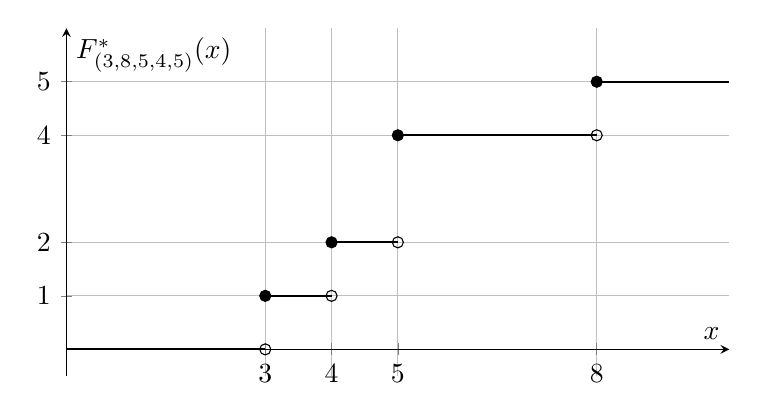
\begin{tikzpicture}
        \begin{axis}[
            axis lines=middle,
            xlabel={$x$},
            ylabel={$F_{(3,8,5,4,5)}^\ast (x)$},
            ymin=-0.5, ymax=6,
            xmin=0, xmax=10,
            xtick={3,4,5,8},
            ytick={0,1,2,4,5},
            grid=both,
            width=10cm,
            height=6cm
        ]

        % Tramos de la función
        \addplot[domain=0:3, thick] {0};

        \addplot[domain=3:4, thick] {1};
        \addplot[domain=4:5, thick] {2};
        \addplot[domain=5:8, thick] {4};
        \addplot[domain=8:10, thick] {5};

        % Puntos abiertos y cerrados
        \addplot[only marks, mark=o] coordinates {(3,0) (4,1) (5,2) (8,4)};
        \addplot[only marks, mark=*] coordinates {(3,1) (4,2) (5,4) (8,5)};

        \end{axis}
        \end{tikzpicture}
        \caption{Representación gráfica de $F_{(3,8,5,4,5)}^\ast (x)$.}
    \end{figure}
\end{ejercicio}

\begin{ejercicio}
    Sea $X$ una variable aleatoria con distribución $B(1,p)$ con $p\in (0,1)$. Se toma una muestra de tamaño 5, $(X_1, X_2, X_3, X_4, X_5)$, y se obtiene la siguiente observación $(0,1,1,0,0)$. Determinar el valor de los estadísticos estudiados en la observación.\\

    \noindent
    Aplicando las fórmulas vistas en clase obtenemos:
    \begin{itemize}
        \item Media: $0.4$.
        \item Varianza: $0.24$.
        \item Cuasivarianza: $0.3$.
        \item $x_{(1)} = 0$, $x_{(2)} = 0$, $x_{(3)} = 0$, $x_{(4)} = 1$, $x_{(5)} = 1$.
    \end{itemize}
\end{ejercicio}

\begin{ejercicio}
    Sea $(X_1, \ldots, X_n)$ una m.a.s. y $\overline{X} = \dfrac{1}{n}\sum\limits_{i=1}^{n}X_i$, entonces:
    \begin{equation*}
        M_{\overline{X}}(t) = {(M_X(\nicefrac{t}{n}))}^{n}
    \end{equation*}

    \begin{equation*}
        M_{\overline{X}}(t) = E\left[e^{t\overline{X}}\right] = E\left[e^{\frac{t}{n}\sum\limits_{i=1}^{n}X_i}\right] = M_{\sum\limits_{i=1}^{n}X_i}\left(\frac{t}{n}\right) \stackrel{\text{indep.}}{=} \prod_{i=1}^{n} M_{X_i}\left(\frac{t}{n}\right) \stackrel{\text{id. d.}}{=} {\left(M_X\left(\frac{t}{n}\right)\right)}^{n}
    \end{equation*}
\end{ejercicio}

\begin{ejercicio}
    Obtener la distribución muestral de $\overline{X}$ para $(X_1, \ldots, X_n)$ una m.a.s. de $X\rightsquigarrow \cc{N}(\mu, \sigma^2)$.

    \begin{equation*}
        M_{\overline{X}}(t) = {\left(M_X\left(\frac{t}{n}\right)\right)}^{n} = {\left(e^{\mu t + \frac{\sigma^2 t^2}{2n^2}}\right)}^{n} = e^{\mu t + \frac{\sigma^2 t^2}{2n}}
    \end{equation*}
    Luego $\overline{X}\rightsquigarrow \cc{N}\left(\mu, \frac{\sigma^2}{n}\right)$, ya que la función generatriz de momentos caracteriza la distribución.
\end{ejercicio}

\begin{prop}
    Si tenemos una m.a.s. $(X_1, \ldots, X_n)$, entonces:
    \begin{align*}
        F_{X_{(n)}}(x) &= {(F_X(x))}^{n} \qquad \forall x\in \mathbb{R} \\
        F_{X_{(1)}}(x) &= 1-{(1-F_X(x))}^{n}
    \end{align*}
    \begin{proof}
        Para la distribución del máximo:
        \begin{align*}
            F_{X_{(n)}}(x) &= P[X_{(n)} \leq x] = P[X_1 \leq x, \ldots, X_n \leq x] \stackrel{\text{indep.}}{=} \prod_{i=1}^{n} P[X_i \leq x] \\ &\stackrel{\text{id. d.}}{=} \prod_{i=1}^{n} P[X\leq x] = {(F_X(x))}^{n}
        \end{align*}
        Para la del mínimo:
        \begin{align*}
            F_{X_{(1)}}(x) &= P[X_{(1)}\leq x] = 1-P[X_{(1)} > x] = 1-P[X_1 > x, \ldots, X_n > x] \\ &\stackrel{\text{indep.}}{=} 1 - \prod_{i=1}^{n}P[X_i > x] \stackrel{\text{id. d.}}{=} 1-{(P[X>x])}^{n} = 1-{(1-F_X(x))}^{n}
        \end{align*}
    \end{proof}
\end{prop}

\begin{ejercicio}
    Obtener las distribuciones muestrales de $X_{(1)}$ y  $X_{(n)}$ para \newline $X\rightsquigarrow U(a,b)$.\\

    \noindent
    Si $X\rightsquigarrow U(a,b)$, entonces:
    \begin{equation*}
        F_X(x) = \dfrac{x-a}{b-a} \qquad \forall x\in [a,b]
    \end{equation*}
    Por lo que aplicando la Proposición superior:
    \begin{align*}
        F_{X_{(n)}}(x) &= {(F_X(x))}^{n} = {\left(\dfrac{x-a}{b-a}\right)}^{n} \qquad \forall x\in [a,b] \\
        F_{X_{(1)}}(x) &= 1 - {(1-F_X(x))}^{n} = 1-{(1-F_X(x))}^{n} = 1-{\left(1-\dfrac{x-a}{b-a}\right)}^{n} \\
                       &= 1-{\left(\dfrac{b-x}{b-a}\right)}^{n} \qquad \forall x\in [a,b]
    \end{align*}
\end{ejercicio}
